\documentclass{ximera}

\author{Jeffrey Kuan}
\input{../preamble} %% Loads the graphics path
\title{Introducton to Quantum Groups and Yang-Baxter Equation For Probabilists}
\license{CC: 0}
\begin{document}
%\begin{abstract}
%    The Yang--Baxter equation is cool. 
%\end{abstract}
%\maketitle
%\part{Introduction}
%\chapterstyle
%    \activity{basics/basicWorksheet}
%    \sectionstyle
%    \activity{basics/exercises/someExercises}

%    \chapterstyle
%    \activity{basics/graphicsInteractives}
\section{Introduction}

Broadly speaking, \textbf{integrable probability} is a branch of probability theory which studies 
models which have exact solutions. For this reason, these models are often called \textbf{exactly solvable.}
From these exact solutions, one can derive precise \textbf{universal} asymptotics, such as the 
famed Tracy--Widom distribution. The origin of these solutions are usually due to algebraic symmetries 
underlying the model. In these set of lecture notes, we will introduce the relevant algebraic background
with a probabilistic researcher as the target audience. 

For historical context, the terminology originates in integrable systems from Hamiltonian mechanics.
In Hamiltonian mechanics, the phase space is represented as a smooth manifold with even dimension $2n,$
with coordinates denoted $q_1,\ldots,q_n,p_1,\ldots,p_n$ for the momentumm and position. An integrable
system is a system with $n$ conserved quantities, and then Liouville--Arnold theorem states that the 
equations of motioni can be solved in quadratures. For an explicit example, the harmonic oscillator in 
one dimension (imagine an object attached to a frictionless spring) is integrable, and the conserved quantity
is the total energy. In contrast, the three--body problem is not integrable, and its solutions are 
notoriously non--exact. 

During the 1980s, many Soviet mathematicians and physicsts introduced quantum mechanics into integrable
systems. In quantum mechanics, quantities such as position, momentum and energy became operators which 
generally do not commute; additionally, the values of these quantities only take discrete, ``quantized''
values. In this context, the concept of ``conserved quantities'' becomes ``commuting operators,'' and 
values of the quantities are eigenvalues of eigenstates. At the time, their approaches were called the
``quantum inverse scattering method.'' Since then, the method has been generalized to abstract 
algebraic objects, such as Hopf algebras. 

These notes will introduce one such algebraic object, known as \textbf{quantum groups,} with a particular
focus on the Yang--Baxter equation. The exposition will use probability and mathematical physics as a
motivation. The goal is for a reader with a probability background to be able to read contemporary (as of
2024) research papers in integrable probability. 

\textbf{Acknolwedgements.} The author was supported by the London Mathematical Society. 

\section{ASEP, XXZ, and $U_q(sl_2)$}

To begin to motivate the notes, we first introduce the asymmetric simple exclusion process (ASEP) and its relationship to 
the Heisenberg XXZ model and the quantum group $U_q(sl_2).$ In ASEP, particles randomly jump on a lattice, which we assume to be
one--dimensional. At most one particle may occupy a site, and jumps to occupied sites are blocked (hence the term ``exclusion'').
Jumps are nearest neighbour (hence the term ``simple''). If the jumps are continuous--time exponential 
clocks with left rates $\alpha$ and right rates $\beta,$ then let $q=\sqrt{\beta/\alpha$} denote the 
asymmetry parameter. If $q\neq 1,$ then the model is asymmetric (sometimes partially asymmetric), 
while for $q=1$ the model is symmetric. For $q=0$ or $q=\infty$ the model is called totally asymmetric.
The symmetric exclusion process (without the word simple) can be defined more generally on an arbritrary graph. In princple, so can 
the asymmetric exclusion process, although this is not as well studied.  

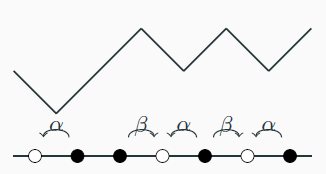
\includegraphics{ASEPScreenshot.png}

The generator of the simple exclusion process can be explicitly written. In the most elementary case 
where there are two lattice sites, then there are four possible configurations. Associate to each
particle the vector $[1\ 0]$ and to each hole (i.e. a non--particle) the vector $[0 \ 1].$ Tensoring
the vectors together, we can associate to each configuration a canonical basis element of the four--dimensional
vector space $\mathbb{C}\otimes \mathbb{C}.$ The field here is chosen to be the complex numbers because
it is algebraically closed, although of course probabilities are real numbers. 

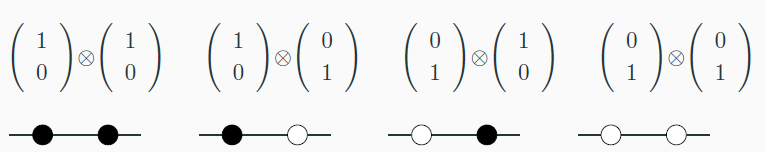
\includegraphics{ASEPConfigurations.png}

With that set up, the generator is then a $4\times 4$ matrix
$$
\alpha\left(
    \begin{array}{cccc}
       0 & 0 & 0 & 0 \\
       0 & -1 & 1 & 0 \\
       0 & q^2 & -q^2 & 0 \\
       0 & 0 & 0 & 0 
    \end{array}
\right)
$$





\end{document}